% !TEX TS-program = pdflatex
% !TEX root = ../tesi.tex

%************************************************
\chapter{Sound design workflow}
\label{chp:intro}
%************************************************

Although is complex to predict the actions of a video game, is possible to control the player's emotions as we want, all this is made possible only by music: the primordial language that regulates the emotional genesis of each person.
There are, obviously, several parameters for making an overall evaluation of the audio implementation for a video game, which concerns both the form and the accuracy of the sounds.
But the parameter of evaluation changes when changing the type and the style of the game too.
The composer and sound designer Brian Schmidt, who worked on tons of games such as NARC, talking about the audio implementation for Arcade games, said:
\begin{flushright}
	\itshape
	Althought games were short, they'd often have a lot of different modes or mini-game \\
	within them, each requiring their own music. \\
	So even a simple painball machine game would have a good 25-30 minutes of interactive original score\\
	\medskip
	--- Brian Schmidt
\end{flushright}

Just as, as far as can be deduced from his words, arcade games have their specific needs for sound design and music composition, in the same way, every different type of video game has its specific needs, let's talk about some of these:

	\paragraph{Scrolling} This type is identified in video games that go in one direction, without level or scene changing. Typically, the sound design is easier, because in just one scene the materials and the actions are ever the same. Isn't the same for the music composition: in this type of videogame the music has to change continuously depending on some element, such as the number of enemies, the level of the health of the main character, the fighting moment, and something else. the main sub-genre of this type of games are:

		\begin{compactitem}
			\item Maze-Chase Games, such as Pac-Man(1982). A game in wich the main character navigate through a maze
			\item Platform games, such as Donkey Kong(1981). A game in wich the main character jump or move from platform to platform
			\item Shot'em Ups, such as Centipede(1981). In wich the main character have a gun to kill every enemy
		\end{compactitem}

	\begin{figure}[h]
		\begin{center}
			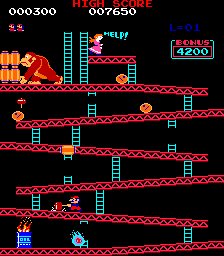
\includegraphics[width=.8\textwidth]{DK.png}
			\caption{the Scrolling Platform game Donkey Kong (1981)}
		\end{center}
	\end{figure}

	\paragraph{Games with levels} Have different needs. The music must change for each scene, as well as the character of the sound design based on the materials used and the soundscape of the scene: a noisy bar, a quiet forest, and an empty room. Each of these environments generates different soundscapes that sound design must adapt to.

The video-game chosen for this implementation is a \textbf{level based game} in first person. Now let's talk about the main elements of an accurate sound design for this type of game.

\section{Polishing}

A player's actions move a video game in one direction rather than another. Is essential to provide feedback to the player based on the importance of the action performed. Music and sounds are essential to guide the player to make choices within the video game. Polishing is an integral part of the ability to capture and immerse the player in the virtual dimension of the game. The dynamics of sound play a fundamental role in this: a good sound designer must be able, through gain staging, to capture the player's attention on the actions performed
In the implementation of this work, that's an alternative approach in the parameter of polishing: There isn't a great work of gain staging, but on the character of the sounds: the more a musical gesture is detached from the traditional idea of ​​sound design, the greater the player's involvement will be. It's a game of expectations: therefore I worked more by abstraction than by causality when I needed to bring the player's attention through an action

\section{Mix}
The balance of frequencies in the sound design image is another important item. Its main goals are 2:

\begin{itemize}
	\item To balance the timbre of the overall audio
	\item To prepare the player's ear for twists and turns
\end{itemize}

Mixing sounds to give roles to each of them in the frequency spectrum best distributes sound energy.
As already mentioned, the durations of the musical gestures are deliberately prolonged and dispersive compared to a traditional approach. This factor certainly doesn't respect the idea of ​​giving a "role" to each sound. However, the material is equalized to maintain at least the "timbral" role of each sound.

\section{Levels of action}
For a sound designer, is useful to find order: spectrally and dynamically distinguish the sounds belonging to the different levels of action: background, actions, and events.

\paragraph{Background sound} are identified in the soundscape. For example, if the main scene is a forest, the background sounds will be the birds, the wind, or the leaves. Despite in this work there isn't a great distinction in the gesture of the implementation, is respected a simple hierarchy structure, giving the role of "background" sounds to the music carpet: an electroacoustic simple immersive flow of many types of timbres.

\paragraph{Actions sound} are related to the direction of the main character: footsteps, pick-up objects, etc. In this implementation, these are the closest sounds to those of a traditional sound design. Not so much for the timbre of the sounds as for their duration, because, since there are short and continuous actions, I couldn't have associated complex musical gestures with them: I need simple and short sounds that are not repetitive, even though they repeat themselves continuously. So I opted for classic electroacoustic glitch sounds, applying random modulations on different parameters (such as volume, pitch, LowPass, and HighPass filter, etc) and inserting them in a random container. In this way, they will always sound different, even though the sounds used for these gestures, such as footsteps, for example, are only 3
\paragraph{Events sounds} are the most important for the involving of the player in the game. For these reason, in this implementation, these sound are the loudest. In the most chase, they are short and loud impulses.

\section{differences between the implementation of sound for game and movies}
The main difference between implementing audio for games and movies is the linearity: a movie has its timeline in which events are located. A film sound designer or composer knows the order of the events and when each one begins and ends, so he has a timeline to follow for adding sounds, gestures, and music in a specific order. A game sound designer must be able to make short and functional gestures, trying to predict which sounds will overlap. Every sound and every music theme must be able to fit with another one, because after a battle scene for example, anything could happen, distorting the mood of the context, precisely because of the non-linearity of the events.

\begin{comment}\begin{code}
\documentclass[\meta{\dots\unkern}]{scrreprt} % or scrbook or scrartcl

\usepackage[\meta{\dots\unkern}]{classicthesis}
\usepackage{arsclassica}

\begin{document}
\dots
\end{document}
\end{code}

For example, this document has been produced with the following code:
\begin{code}
\documentclass[a4paper,twoside,openright,titlepage,
               headinclude,footinclude,BCOR5mm,
               numbers=noenddot,cleardoublepage=empty,
               tablecaptionabove]{scrreprt}

\usepackage{\meta{\dots\unkern}}
\usepackage{subfig}
\usepackage[eulerchapternumbers,subfig,beramono,eulermath,pdfspacing]%
           {classicthesis}
\usepackage{arsclassica}

\begin{document}
\dots
\end{document}
\end{code}

It is recommended to use the \optname{beramono} and \optname{eulerchapternumbers} options together with \arsclassica.



\section{Style}

The typographical style achieved with \arsclassica{} differs from \classicthesis{} in the following points:
\begin{itemize}
\item use of Iwona font, by Janusz Nowacki, for the sectioning unit titles (chapters, sections, subsections, sub-subsections, paragraphs and subparagraphs), for the description list labels, the headlines and the caption labels (\classicthesis{} doesn't use any sans serif font);
\item customized chapter numbers;
\item semi-transparent headlines; the headlines are separated from the page number by a small rule;
\item caption labels in boldface (\classicthesis{} doesn't use any boldface font);
\item itemize lists with semi-transparent bullets.
\end{itemize}

\arsclassica{} is designed  to provide a ready-to-use typographical style: for this reason it has no loading options and it is \emph{not} configurable or customizable in any way. If you change the previous settings, you'll risk to destroy the balance of the style, so it is \emph{highly recommended} to keep them unchanged.

One of the principles of \LaTeX{} is that it allows the author to take no interest in the typographical questions, permitting him to focus only on the structure and the contents of his document. This fact should always be kept in mind: using a style written by others, the user accepts all the typographical settings chosen for him by the author of the style, and he isn't forced to study typography to fine-tune the layout of his publications. This is the case of \arsclassica{} too: if you change its settings, you'll deny this philosophy and, consequently, you'll have to study (a lot of) typography to achieve acceptable results.

The style achieved with \arsclassica{} is \emph{not} therefore configurable or customizable. The typographical style is very personal: if you like this package and find attractive the idea to take no interest in the problem of the style definition, then you'll use \arsclassica{} with satisfaction; otherwise, if you have different needs or you aren't satisfied with the layout of the package, then you should try other classes or packages, even building your own style.



\section{Important}

To write a document according to the \arsclassica{} style, you have to follow some very simple rules.
\begin{itemize}
\item Don't change \emph{for any reason} the \arsclassica{} settings (fonts, text body size, colors, \dots).
\item The sectioning unit titles (chapters, section, subsections, \dots) have to be \emph{one line long}, possibly in \emph{plain text} (no symbols, formulas or code fragments). If you have titles longer than one line, try and rephrase them: you can almost always do it.
\item In the table of contents and in the list of tables and figures, captions have to be \emph{one line long}, possibly in \emph{plain text}. Use the optional argument of sectioning commands and of \cmdname{caption}, if necessary.
\item Don't use \optname{tocaligned} and \optname{dottedtoc} options of \classicthesis: the default table of contents does the job very well (see the documentation of \classicthesis{} for a nice discussion of this point).
\item Don't use vertical or double rules in your tables (see the documentation of \pkgname{booktabs}).
\item Use footnotes and margin notes very sparingly.
\item If your document includes graphs and plots, draw them using \LaTeX{} (by \pkgname{Ti\emph{k}Z} and \pkgname{pgfplots}, for example) and not an external software. This is the only way to get the best typographical outcome.
\end{itemize}



%\section{Examples}
%intendo sostituire queste immagini con qualcuna inerente al mio progetto
\begin{figure}
\centering
\subfloat[Asia personas duo]
{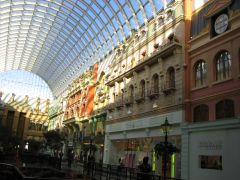
\includegraphics[width=.45\columnwidth]{Lorem}} \quad
\subfloat[Pan ma signo]
{\label{fig:example-b}%
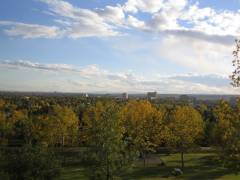
\includegraphics[width=.45\columnwidth]{Ipsum}} \\
\subfloat[Methodicamente o uno]
{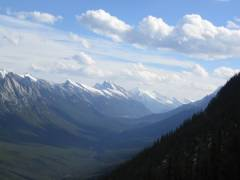
\includegraphics[width=.45\columnwidth]{Dolor}} \quad
\subfloat[Titulo debitas]
{
\includegraphics[width=.45\columnwidth]{Sit}}
\caption[Tu duo titulo debitas latente]{Tu duo titulo debitas latente}
\label{fig:example}
\end{figure}
Please note that the content of this section is just some dummy text. It isn't a real language.

Lorem ipsum dolor sit amet, consectetuer adipiscing elit. Ut purus elit, vestibulum ut, placerat ac, adipiscing vitae, felis. Curabitur dictum gravida mauris.

\subsection*{A subsection}

\lipsum[2]

\subsubsection*{A sub-subsection}

\lipsum[7]

\paragraph{A paragraph}
Lorem ipsum dolor sit amet, consectetuer adipiscing elit. Ut purus elit, vestibulum ut, placerat ac, adipiscing vitae, felis. Curabitur dictum gravida mauris. Nam arcu libero, nonummy eget, consectetuer id, vulputate a, magna.

\paragraph{Another paragraph}
Cras nec ante, pellentesque a nulla, cum sociis natoque penatibus et magnis dis parturient montes, nascetur ridiculus mus. Aliquam tincidunt urna

\bigskip

Donec aliquet, tortor sed accumsan bibendum, erat ligula aliquet magna, vitae ornare odio metus a mi. Morbi ac orci et nisl hendrerit mollis. Suspendisse ut massa. Cras nec ante. Pellentesque a nulla. Cum sociis natoque penatibus et magnis dis parturient montes, nascetur ridiculus mus. Aliquam tincidunt urna.

\begin{description}
\item[Mane] Lorem ipsum dolor sit amet, consectetuer adipiscing elit.
\item[Tekel] Ut purus elit, vestibulum ut, placerat ac, adipiscing vitae, felis. Curabitur dictum gravida mauris.
\item[Fares] Nam arcu libero, nonummy eget, consectetuer
id, vulputate a, magna.
\end{description}

\begin{table}
\caption{Lorem ipsum dolor sit amet}
\centering
\begin{tabular}{ll}
\toprule
\textbf{Alkaloid} & \textbf{Origin} \\
\midrule
atropine & belladonna \\
morphine & poppy \\
nicotine & tobacco \\
\bottomrule
\end{tabular}
\end{table}

Suspendisse vel felis. Ut lorem lorem, interdum eu, tincidunt sit amet, laoreet vitae, arcu. Aenean faucibus pede eu ante. Praesent enim elit, rutrum at, molestie non, nonummy vel, nisl. Ut lectus eros, malesuada sit amet, fermentum eu, sodales cursus, magna. Donec eu purus. Quisque vehicula, urna sed ultricies auctor, pede lorem egestas dui, et convallis elit erat sed nulla.

\subsection*{Some formulas}

Una formula in linea viene incorporata nel testo: $\lim_{n \to \infty}\sum_{k=1}^n \frac{1}{k^2} = \frac{\pi^2}{6}$, per esempio. Come si osserva, \LaTeX{} fa \emph{il possibile} per comprimerla e modificare il meno possibile l'interlinea nel capoverso che la contiene.
Una formula in display viene invece composta da \LaTeX{} su linee a parte, separate dal contesto con adeguati spazi bianchi per metterla in mostra e farla risaltare sulla pagina.
\begin{equation}
\lim_{n \to \infty}\sum_{k=1}^n \frac{1}{k^2}= \frac{\pi^2}{6}
\end{equation}
Come si osserva, ora la formula risulta centrata, non compressa, e tutti i suoi elementi occupano il giusto spazio con un risultato finale di grande respiro.

Integer tempus convallis augue. Etiam facilisis. Nunc elementum fermentum wisi. Aenean placerat. Ut imperdiet, enim sed gravida sollicitudin, felis odio placerat quam, ac pulvinar elit purus eget enim.

\begin{equation}
\int_a^{a+T}f(x)\,dx= \int_0^T f(x)\,dx
\qquad
\oint f(z)\,dz=2\pi i
\end{equation}

Nulla malesuada porttitor diam. Donec felis erat, congue non, volutpat at, tincidunt tristique, libero. Vivamus viverra fermentum felis. Donec non- ummy pellentesque ante.

\begin{equation}
f(x_1,\dots,x_n)=  \prod_{k=1}^n x_k
\qquad
\sum_{k=1}^n x_k^2=1
\qquad
\biggl(\sum_n x_n^2\biggr)^{1/2}
\end{equation}

\lipsum[2]

\begin{equation}
\begin{bmatrix}
a_{11} & \dots & a_{1n} \\
a_{21} & \dots & a_{2n} \\
\hdotsfor{3} \\
a_{n1} & \dots & a_{nn}
\end{bmatrix}
\end{equation}

\lipsum[4]

\begin{equation}
\lim_{x\to 0}
\frac{\sin x}{x}=1 \qquad
\lim_{n\to +\infty}f_n=\delta
\end{equation}

Fusce mauris. Vestibulum luctus nibh at lectus. Sed bibendum, nulla a faucibus semper, leo velit ultricies tellus, ac venenatis arcu wisi vel nisl. Vestibulum diam.

\begin{equation}
n!=
\begin{cases}
1       & \text{if $n=0$} \\
n(n-1)! & \text{if $n\ge 1$}
\end{cases}
\end{equation}

Ut lectus eros, malesuada sit amet, fermentum eu, sodales cursus, magna. Donec eu purus. Quisque vehicula, urna sed ultricies auctor, pede lorem egestas dui, et convallis elit erat sed nulla. Donec luctus. Curabitur et nunc. Aliquam dolor odio, commodo pretium, ultricies non, pharetra in, velit.

\begin{equation}
x_G=
\frac{\displaystyle
      \sum_{i=1}^n m_ix_i}
{\displaystyle\sum_{i=1}^n m_i}
\end{equation}

\lipsum[6]

\begin{equation}
\kappa =\frac{\xi}{E_{\textrm{max}}}
\qquad
E_{\textup{max}} =\frac{2 m_{\textup{e}} \beta^2\gamma^2 }{1 +2\gamma m_{\textup{e}}/m_{\textrm{x}} + ( m_{\textup{e}}/m_{\textup{x}})^2}
\end{equation}

\lipsum[8]
\end{comment}
